\documentclass[11pt,letterpaper,titlepage]{article}

%================== Document nomenclature
\newcommand{\DOCSUBJT}{Whitepaper: }   %Put document subject here
\newcommand{\DOCTITLE}{                      %Put document title here
	The Monte-Carlo Solver in ChiTech
}       
\newcommand{\DOCDATE} {August, 2019}         %Put document date here
\newcommand{\DOCREV}  {Rev 1.00}             %Put revision number here

%================== Misc Settings
\usepackage{fancyhdr}
\usepackage[left=0.75in, right=0.75in, bottom=1.0in]{geometry}
\usepackage{lastpage}
\usepackage{titleref}
\usepackage{booktabs}
\usepackage{appendix}
\usepackage{ stmaryrd }

\appendixtitleon
\appendixtitletocon

\makeatletter

%================== List of figures and tables mods
\usepackage{tocloft}
\usepackage[labelfont=bf]{caption}

\renewcommand{\cftfigpresnum}{Figure\ }
\renewcommand{\cfttabpresnum}{Table\ }

\newlength{\mylenf}
\settowidth{\mylenf}{\cftfigpresnum}
\setlength{\cftfignumwidth}{\dimexpr\mylenf+1.5em}
\setlength{\cfttabnumwidth}{\dimexpr\mylenf+1.5em}



%=================== Graphics
\usepackage{graphicx}
\usepackage[breakwords]{truncate}
\usepackage{float}
\usepackage{array}
\usepackage{amsmath}
\usepackage{mdframed}
\usepackage{fancyvrb}
\usepackage{float}
\usepackage{cancel}
\usepackage{amssymb}
\graphicspath{ {images/} }
\usepackage[usenames,dvipsnames,svgnames,table]{xcolor}
\usepackage[defaultlines=2,all]{nowidow}
\usepackage{listings}
\usepackage{color}
\definecolor{Brown}{cmyk}{0,0.81,1,0.60}
\definecolor{OliveGreen}{cmyk}{0.64,0,0.95,0.40}
\definecolor{CadetBlue}{cmyk}{0.62,0.57,0.23,0}
\usepackage{pdflscape}
\usepackage{relsize}
\usepackage{verbatim}
\usepackage{tabto}
\usepackage{upgreek}
\usepackage{enumitem}

\usepackage{mathtools}

%=================== Settings
\renewcommand{\baselinestretch}{1.2}
\definecolor{gray}{rgb}{0.4 0.4 0.4}
\newcommand{\stimes}{{\times}}

\newcommand*{\ldblbrace}{\{\mskip-5mu\{}
\newcommand*{\rdblbrace}{\}\mskip-5mu\}}


\newcommand{\xmltag}[1]{\textcolor{blue}{ \texttt{#1}} }
\newcommand{\xmloption}[1]{\textcolor{ao(english)}{ \texttt{#1}} }

%================== Code syntax highlighting
\lstset{language=C++,frame=ltrb,framesep=2pt,basicstyle=\linespread{0.8} \small,
	keywordstyle=\ttfamily\color{OliveGreen},
	identifierstyle=\ttfamily\color{CadetBlue}\bfseries,
	commentstyle=\color{Brown},
	stringstyle=\ttfamily,
	showstringspaces=true,
	tabsize=2,}
	
%=================== Big cdot
\newcommand*\bigcdot{\mathpalette\bigcdot@{.5}}
\newcommand*\bigcdot@[2]{\mathbin{\vcenter{\hbox{\scalebox{#2}{$\m@th#1\bullet$}}}}}

\newcommand{\beq}{\begin{equation*}
\begin{aligned}}
\newcommand{\eeq}{\end{aligned}
\end{equation*}}

\newcommand{\beqn}{\begin{equation}
	\begin{aligned}}
\newcommand{\eeqn}{\end{aligned}
	\end{equation}}

\newcommand{\bOmega}{\mathcal{D}}

\setlength\parindent{0pt}

%================== Section numbers with equation numbers
\numberwithin{equation}{section}

\begin{document}

\begin{titlepage}
	\pagestyle{fancy}
	\vspace*{1.0cm}
	\centering
	\vspace{1cm}
	\vspace{.25cm}
	{\Large\bfseries  \DOCSUBJT \par} 
	{\Large\bfseries \DOCTITLE  \par}
	\vspace{1cm}
	{\Large \DOCDATE \par}
	\vspace{1.0cm}
	{\Large Jan Vermaak \par}
	{\Large \DOCREV \par}
	\begin{center}
		\begin{minipage}[c]{0.45\textwidth}
			\begin{figure}[H]
				
				
\includegraphics[width=3in]{Figures/Logo2_Medium.png}
			\end{figure}
		\end{minipage}
	\end{center}

\end{titlepage}	


\pagestyle{fancy}
\rfoot{Page \thepage \ of \pageref{LastPage}}
\cfoot{}
\lfoot{\truncate{14cm}{\DOCTITLE}}
\rhead{}
\chead{\currentname}
\lhead{}
\renewcommand{\footrulewidth}{0.4pt}

\begin{comment}
\tableofcontents
\addtocontents{toc}{~\hfill\textbf{Page}\par}

\listoffigures
\listoftables

\end{comment}


%#########################################################################
\newpage
\chead{Basic transport}	
\section{Basic transport}
The fundamental transport of a particle in a medium, where the interaction probability is given by $\sigma_t$ in units $[cm^{-1}]$, can be described as follows. Given a flux of particles, $\phi$, in units $[cm^{-2}s^{-1}]$ the interaction rate per unit volume is given by

\beq
RR = \sigma_t \phi
\eeq
\newline
This also represents the rate of change of $\phi$ as

\beq
\frac{d\phi}{dx} = - \sigma_t \phi
\eeq
\newline
This forms a first order differential equation which we can multiply with the integration factor $e^{\sigma_t x}$

\beq
e^{\sigma_t x} \frac{d\phi}{dx} + \sigma_t e^{\sigma_t x} \phi = 0 \\
\therefore
\frac{d}{dx} \biggr(  e^{\sigma_t x} \phi \biggr) = 0 \\
\int_0^L \frac{d}{dx} \biggr(  e^{\sigma_t x} \phi \biggr).dx = 0 \\
\biggr(  e^{\sigma_t x} \phi \biggr)_0^L = 0\\
e^{\sigma_t L}\phi_L - \phi_0 = 0 \\
\therefore 
\frac{\phi_L}{\phi_0} = e^{-\sigma_t L}
\eeq
\newline
The amount of interactions in distance $L$ is then given by $\phi_0 - \phi_L$, and the probability of interacting, $p_i$ within the distance $L$ is given by

\beq 
p_i = \frac{\phi_0-\phi_L}{\phi_0} = 1 - \frac{\phi_L}{\phi_0} \\
\therefore
p_i = 1 - e^{-\sigma_t L}
\eeq 
\newline
This form of the interaction probability is a curve which starts at zero and assymptotically tends to unity. Additionally, this equation can be inverted by solving for L

\beq
e^{-\sigma_t L} = 1 - p_i \\
-\sigma_t L = ln(1-p_i) 
\eeq 
\beqn
\therefore
L = -\frac{ln(1-p_i)}{\sigma_t}
\eeqn
\newline
This equation can now be sampled in a given material by randomly sampling $p_i \in [0,1]$ which will produce the distance-to-interaction, $d_i$. We now denote any random number $\theta \in [0,1]$ and write the base equation for sampling the distance-to-interaction

\beqn
d_i = -\frac{ln(1-\theta)}{\sigma_t}
\eeqn  

\vspace{0.5cm}
Consider the multi-zone geometry in \ref{fig:multizonehomo} below. For practical purposes it is important to be able to resample the distance-to-interaction from one zone to another. The question is however if the resampling of a multi-zone geometrical arrangement is equivalent to a single large zone. It can be proved statistically that the two sampling techniques are equivalent.

\begin{figure}[H]
\centering
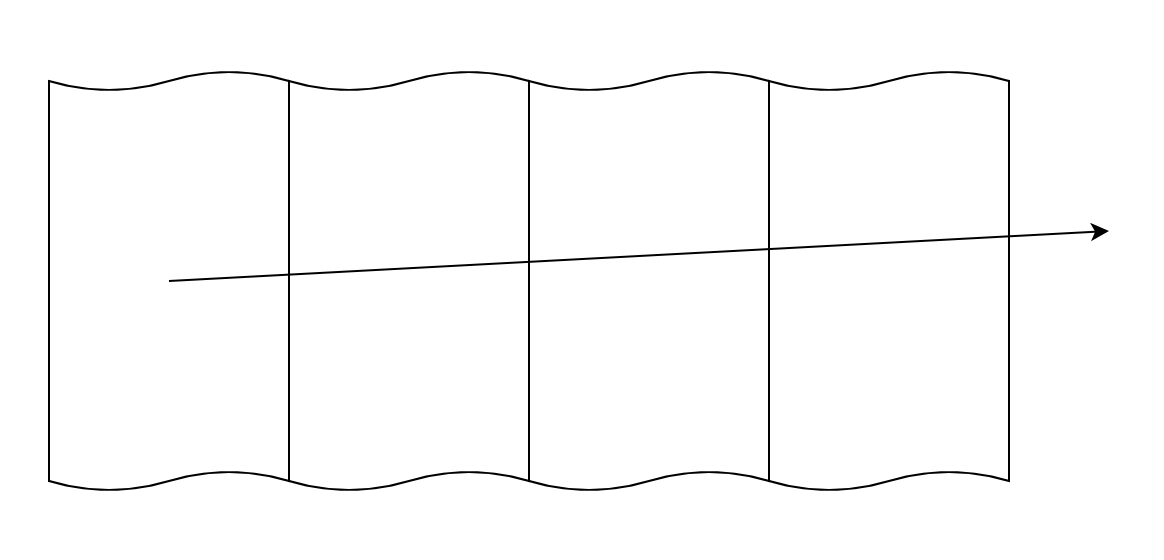
\includegraphics[width=0.7\linewidth]{Figures/MultizoneHomo}
\caption{Multi-zone geometry.}
\label{fig:multizonehomo}
\end{figure}

The next quantity to compute is the distance-to-surface, $d_s$. This process we will call \textbf{ray-tracing}.

\newpage
\chead{Raytracing in slabs}
\section{Raytracing utilities}
\subsection{Intersection of a line and a plane \xmltag{chi\_mesh::CheckPlaneLineIntersect}}
\begin{figure}[H]
\centering
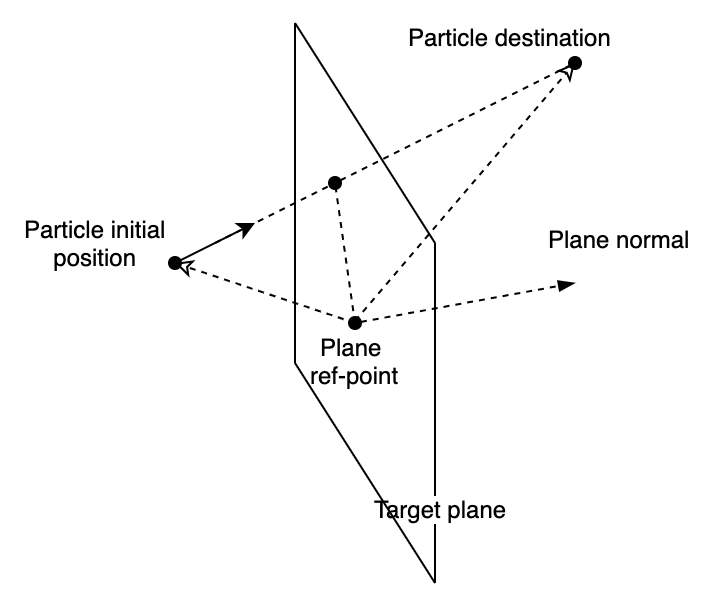
\includegraphics[width=0.4\linewidth]{Figures/MultizoneHomo1}
\caption{Graphical representation of intersection of a line with a plane.}
\label{fig:multizonehomo1}
\end{figure}

Given a particle's location, $\bar{r}_i$, and direction, $\hat{\Omega}$, we can create a 3D line of the form

\beq 
\bar{r} &= \bar{r}_i + d\hat{\Omega} \\
(x,y,z) &= (x_i,y_i,z_i) + d (\Omega_x,\Omega_y,\Omega_z)
\eeq 
\newline
where d is the only unknown parameter required to define $\bar{r} = (x,y,z)$. Alternatively we can be supplied by another point on the line, $\bar{p}_f$ and then define a weight, $w\in [0,1]$, which can define a \textbf{line segment}
\beq 
\bar{r} &= w\bar{r}_i + (w-1)\bar{r}_f\\
(x,y,z) &= w(x_i,y_i,z_i) + (w-1) (x_f,y_f,z_f)
\eeq 
\newline
For the equation of a plane we need a refence point, $\bar{p}_0$, and a normal, $\hat{n}$, after which we can form a vector from point $\bar{p}_0$ to $\bar{r}_p = (x,y,z)$. The plane is then defined by the relationship that the dot-product of this vector with the normal is zero, 

\beq
\hat{n}\bigcdot(\bar{r}_p - \bar{p}_0) = 0 
\eeq 
\beq
n_x(x-p_{0x}) + 
n_y(y-p_{0y})+
n_z(z-p_{0z})=0.
\eeq
\newline
A very simple way to simultaneously determine whether the line intersects the plane and where the intersection is, is to use the segment definition of the line and compute two vectors; one from $\bar{p}_0$ to $\bar{r}_i$, and another from $\bar{p}_0$ to $\bar{r}_f$
\beq
\vec{v}_i = \bar{r}_i - \bar{p}_0 \quad \text{ and } \quad
\vec{v}_f = \bar{r}_f - \bar{p}_0
\eeq 
after which we compute the projection of these vectors along the normal of the plane by taking the dot-products
\beq 
D_i = \hat{n}\bigcdot\vec{v}_i \quad \text{ and } \quad
D_f = \hat{n}\bigcdot\vec{v}_f.
\eeq 
Since we use the same normal for both computations the line is intersecting the plane only if the signs of the dot-products is not equal and $w$ can then be computed as

\beq
\text{if} \quad \text{sgn}(D_i)\ne \text{sgn}(D_f) \\
\eeq
\beq
w = \frac{|D_i|}{|D_i| + |D_f|}
\eeq

\textbf{Implementation}
\begin{lstlisting}[language=c++]
bool chi_mesh::
CheckPlaneLineIntersect(chi_mesh::Normal plane_normal,
                        chi_mesh::Vector plane_point,
                        chi_mesh::Vector line_point_0,
                        chi_mesh::Vector line_point_1,
                        chi_mesh::Vector& intersection_point,
                        std::pair<double,double>& weights)
{
  chi_mesh::Vector v0 = line_point_0 - plane_point;
  chi_mesh::Vector v1 = line_point_1 - plane_point;

  double dotp_0 = plane_normal.Dot(v0);
  double dotp_1 = plane_normal.Dot(v1);

  bool sense_0 = (dotp_0 >= 0.0);
  bool sense_1 = (dotp_1 >= 0.0);

  if (sense_0 != sense_1)
  {
    double dotp_total = std::fabs(dotp_0) + std::fabs(dotp_1);
    weights.first = (std::fabs(dotp_0)/dotp_total);
    weights.second = 1.0 - weights.first;
    intersection_point =
      line_point_0*weights.second +
      line_point_1*weights.first;

    return true;
  }

  return false;
}
\end{lstlisting}

\newpage
\chead{References}
\begin{thebibliography}{1}
    
    \bibitem{blender} {\em Blender - a 3D modelling and rendering package}, Blender Online Community, Blender Foundation, Blender Institute, Amsterdam, 2018
    
    \bibitem{delaunay} Cheng et al, {\em Delaunay Mesh Generation}, Chapman \& Hall/CRC Computer \& Information Science Series, 2013
    
    
\end{thebibliography}





\end{document}